\section{Routing-Atlas}\label{sec:atlas}

Der Routing-Atlas ist ein Projekt der inet AG in Zusammenarbeit mit dem Bundesamt für Sicherheit in der Informationstechnik (BSI), \vgl \cite{waehlisch2010towards,waehlisch2010framework,schmidt2010}.
Angesichts der wachsenden Bedeutung des Internet als kritische Infrastruktur für Wirtschaft, Verwaltung und Bildung und der zunehmenden Regulierung dieses Mediums stellt sich die Frage welche Akteure und Jurisdiktionen Einfluss nehmen können.
Ziel des Projektes ist es landesspezifische Teile des Internet und Abhängigkeiten zwischen Ländern zu identifizieren, zu klassifizieren und zu visualisieren.
Damit kann zum Beispiel abgeschätzt werden:
\begin{itemize}
 \item Zu welchen Akteuren und Ländern bestehen Abhängigkeiten?
 \item Wie stark ist die landesinterne Kommunikation in sich geschlossen?
 \item Wie störbar ist die landesinterne Kommunikation?
 \item Wie leicht lässt sich nationaler Traffic umleiten?
\end{itemize}

Mit ähnlichen Fragenstellungen haben sich bereits Karlin et al.~\cite{0903.3218v1} beschäftigt.
Sie haben hierbei die Zuordnung zu Ländern auf der Basis teils bereits aggregierter IP-Präfixe statt der im Routing-Atlas verwendeten IP-Adressblöcken vorgenommen.

Im Folgenden wird auf die Schritte zur Erstellung des Routing-Atlas eingegangen.

\subsection{Identifikation des "`deutschen Internets"'}
Die Organisation des Internet berücksichtigt politische oder geographische Grenzen nicht.
IP-Adressen, IP-Adressblöcke, IP-Präfixe und Nummern Autonomer Systeme enthalten für sich genommen keine Metainformationen, aus denen auf die Zugehörigkeit zu einem Land oder einer Organisation geschlossen werden kann.
Zur Lösung dieses Problems werden Informationen aus administrativen Datenbanken der Regional Internet Registries (RIR) genutzt.
Die für Europa zuständige RIR ist das Réseaux IP Européens Network Coordination Centre (RIPE NCC)~\cite{RIPE}.
Um möglichst viele Teilnehmer des "`deutschen Internets"' zu identifizieren, werden zunächst IP-Adressblöcke - die kleinsten in der Datenbank vertretenen Entitäten - betrachtet.

Das RIPE NCC vergibt für Europa IP-Adressblöcke und verwaltet diese in einer (weitesgehend) öffentlich zugänglichen Datenbank.
Diese Datenbank wird nach Adressblöcken (\texttt{inetnum}-Objekte) durchsucht, deren \texttt{country}-Attribut 'DE' oder 'EU' ist.
Zu den 'EU' Adressblöcken wird in weiteren Attributen nach Einträgen gesucht, die eine Einordnung als "`deutscher"' Adressblock zulassen.
Beginnt beispielsweise die Telefonnummer einer für den Adressblock verantwortlichen Kontaktperson oder Organisation mit '+49', wird der Adressblock aufgenommen.
Aus datenschutzrechtlichen Gründen limitiert die RIPE den Zugriff auf personenbezogen Daten auf ein Kontingent von einigen Hundert Anfragen pro Tag, sodass einmal abgefragte Informationen zwischengespeichert werden sollten und die Frequenz der Anfragen an die RIPE DB gering gehalten werden muss.

Im nächsten Schritt werden die gefundenen Adressblöcke zu routbaren Präfixen zusammengefasst.
Dazu werden \texttt{route}-Objekte in der RIPE DB gesucht, deren Präfixe die identifizierten Adressblöcke beinhalten.

%\begin{figure}
% \begin{center}
%  \includegraphics[width=0.5\textwidth]{toolchain_fit}
%  \caption{Toolchain: IP-Adressblöcke zu Autonomen Systemen} \label{fig:toolchain_fit}
% \end{center}
%\end{figure}

Die hierbei gefunden \texttt{route}-Objekte haben idR. ein \texttt{origin}-Attribut, dass auf den Datensatz des Autonomen Systems (\texttt{aut-num}-Objekt) verweist.
Fehlt dem Präfix eine Zuordnung zu einem AS, wird eine Auflösung beim Team Cymru und - schlägt auch dies fehl - beim RIPE RIS-Kollektor RRC 12 (DE-CIX in Frankfurt) versucht~\cite{RIPE:RIS, Cymru}.

Durch die Nutzung mehrerer Datenquellen bleiben nur wenige Präfixe ($\approx 2\%$) unaufgelöst.

%\subsection{Klassifikation der ASe}
%TODO

\subsection{Bildung des AS Graphen}
\label{atlas:graph}

Am NEC-Lab wurde im Rahmen eines europäischen Forschungsprojektes ein Modell der Routing-Topologie des Internets auf Ebene der Autonomen Systeme erstellt~\cite{conf/pads/Winter09}.
Hierfür wurden die vom Internet Research Lab der UCLA gesammelten und aggregierten Daten genutzt~\cite{IRLtopology}.
Ein Ergebnis dieses Modells ist die next hop matrix.
Sie beinhaltet für die Wege von einem AS zu einem anderen jeweilse das nächste AS, über das ein Paket geroutet werden würde.
Auf die Generierung der next hop matrix wird in Abschnitt~\ref{sec:winter} eingegangen.

Der Routing-Atlas verwendet die next hop matrix, um einen Graphen aller im vorherigen Schritt identifizierten Autonomen Systeme zu bilden.
Dieser Graph umfasst neben den "`deutschen"' ASen auch jene, die für die Verbindung sorgen und im Ausland liegen - die Transit-ASe.
Analysiert man nun diesen Graphen, so lassen sich Antworten auf die ursprünglichen Fragen nach der Abhängigkeit und Geschlossenheit landesinterner Kommunikation vom Ausland finden.


\subsection{Visualisierung}

Der im vorherigen Schritt erstellte Graph wird graphisch dargestellt.
Da der Gesamtgraph in Auflösungen unterhalb eines wandfüllenden Ausdrucks unübersichtlich ist, werden hierbei hauptsächlich gefilterte Subgraphen dargestellt.
Um weiterhin die Bedeutung einzelner Autonomer Systeme besser zu veranschaulichen, wird die dargestellte Einfärbung, Größe oder Position eines AS nach einer Klassifikation festgelegt.
Aspekte nach denen ein AS klassifiziert wird sind
\begin{itemize}
 \item die Anzahl enthaltener IP-Präfixe oder IP-Adressblöcke,
 \item die hierarchische Einordnung in die Routing-Topologie des Internets,
 \item die Branchenzugehörigkeit.
\end{itemize}

Abbildung~\ref{fig:asgraph_cat10} zeigt die Autonomen Systeme der Branche 'Wissenschaft, Forschung \& Kultur (F\&E)' in einem hierarchischen Kreisdiagramm. Die Position eines AS in diesem Diagramm bedeutet, dass es in seiner topologischen Bedeutung (von innen nach außen) Tier 1, Large ISP, Small ISP und Stub zuzuordnen ist.

%\begin{figure}
% \begin{center}
%  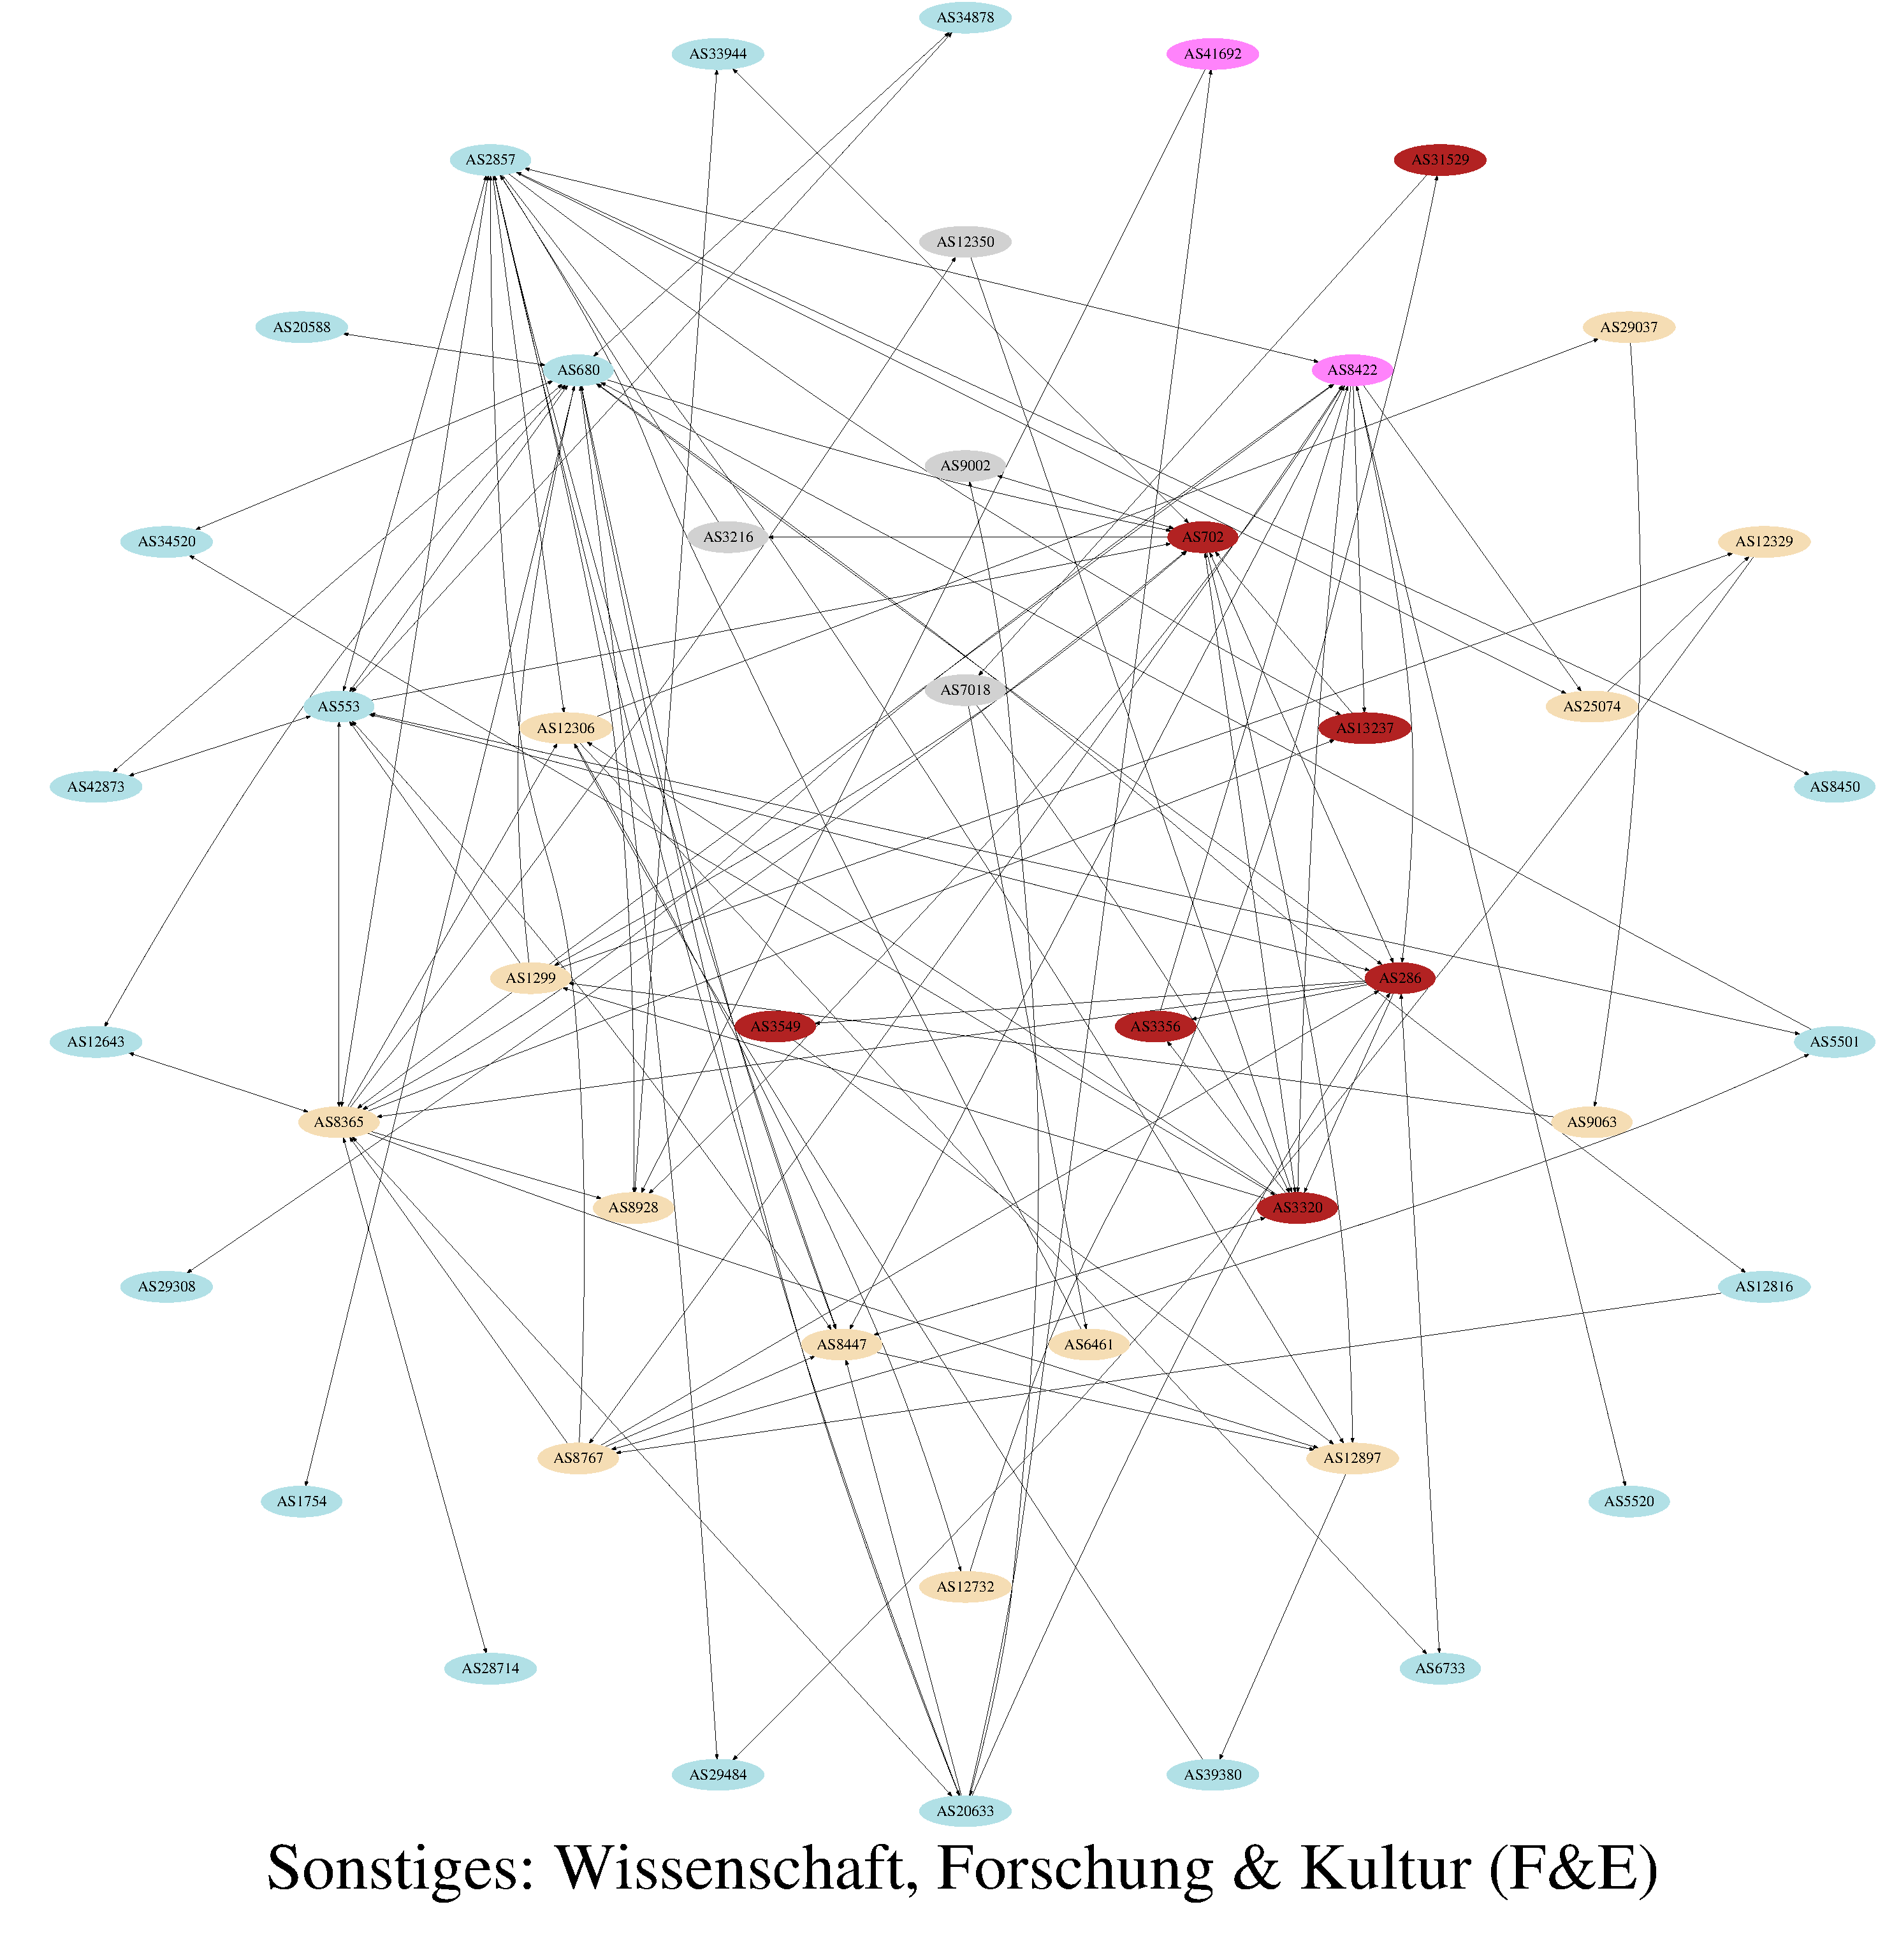
\includegraphics[width=0.55\textwidth]{asgraph_cat10-pos}
%  \caption{Hierarchisches Kreismodell} \label{fig:asgraph_cat10}
% \end{center}
%\end{figure}



